% Generated by Sphinx.
\def\sphinxdocclass{report}
\documentclass[letterpaper,10pt,english]{sphinxmanual}
\usepackage[utf8]{inputenc}
\DeclareUnicodeCharacter{00A0}{\nobreakspace}
\usepackage{cmap}
\usepackage[T1]{fontenc}
\usepackage{babel}
\usepackage{times}
\usepackage[Bjarne]{fncychap}
\usepackage{longtable}
\usepackage{sphinx}
\usepackage{multirow}

\addto\captionsenglish{\renewcommand{\figurename}{Fig. }}
\addto\captionsenglish{\renewcommand{\tablename}{Table }}
\floatname{literal-block}{Listing }



\title{sportfac_project Documentation}
\date{June 11, 2015}
\release{0.1}
\author{ChangeToMyName}
\newcommand{\sphinxlogo}{}
\renewcommand{\releasename}{Release}
\makeindex

\makeatletter
\def\PYG@reset{\let\PYG@it=\relax \let\PYG@bf=\relax%
    \let\PYG@ul=\relax \let\PYG@tc=\relax%
    \let\PYG@bc=\relax \let\PYG@ff=\relax}
\def\PYG@tok#1{\csname PYG@tok@#1\endcsname}
\def\PYG@toks#1+{\ifx\relax#1\empty\else%
    \PYG@tok{#1}\expandafter\PYG@toks\fi}
\def\PYG@do#1{\PYG@bc{\PYG@tc{\PYG@ul{%
    \PYG@it{\PYG@bf{\PYG@ff{#1}}}}}}}
\def\PYG#1#2{\PYG@reset\PYG@toks#1+\relax+\PYG@do{#2}}

\expandafter\def\csname PYG@tok@gd\endcsname{\def\PYG@tc##1{\textcolor[rgb]{0.63,0.00,0.00}{##1}}}
\expandafter\def\csname PYG@tok@gu\endcsname{\let\PYG@bf=\textbf\def\PYG@tc##1{\textcolor[rgb]{0.50,0.00,0.50}{##1}}}
\expandafter\def\csname PYG@tok@gt\endcsname{\def\PYG@tc##1{\textcolor[rgb]{0.00,0.27,0.87}{##1}}}
\expandafter\def\csname PYG@tok@gs\endcsname{\let\PYG@bf=\textbf}
\expandafter\def\csname PYG@tok@gr\endcsname{\def\PYG@tc##1{\textcolor[rgb]{1.00,0.00,0.00}{##1}}}
\expandafter\def\csname PYG@tok@cm\endcsname{\let\PYG@it=\textit\def\PYG@tc##1{\textcolor[rgb]{0.25,0.50,0.56}{##1}}}
\expandafter\def\csname PYG@tok@vg\endcsname{\def\PYG@tc##1{\textcolor[rgb]{0.73,0.38,0.84}{##1}}}
\expandafter\def\csname PYG@tok@m\endcsname{\def\PYG@tc##1{\textcolor[rgb]{0.13,0.50,0.31}{##1}}}
\expandafter\def\csname PYG@tok@mh\endcsname{\def\PYG@tc##1{\textcolor[rgb]{0.13,0.50,0.31}{##1}}}
\expandafter\def\csname PYG@tok@cs\endcsname{\def\PYG@tc##1{\textcolor[rgb]{0.25,0.50,0.56}{##1}}\def\PYG@bc##1{\setlength{\fboxsep}{0pt}\colorbox[rgb]{1.00,0.94,0.94}{\strut ##1}}}
\expandafter\def\csname PYG@tok@ge\endcsname{\let\PYG@it=\textit}
\expandafter\def\csname PYG@tok@vc\endcsname{\def\PYG@tc##1{\textcolor[rgb]{0.73,0.38,0.84}{##1}}}
\expandafter\def\csname PYG@tok@il\endcsname{\def\PYG@tc##1{\textcolor[rgb]{0.13,0.50,0.31}{##1}}}
\expandafter\def\csname PYG@tok@go\endcsname{\def\PYG@tc##1{\textcolor[rgb]{0.20,0.20,0.20}{##1}}}
\expandafter\def\csname PYG@tok@cp\endcsname{\def\PYG@tc##1{\textcolor[rgb]{0.00,0.44,0.13}{##1}}}
\expandafter\def\csname PYG@tok@gi\endcsname{\def\PYG@tc##1{\textcolor[rgb]{0.00,0.63,0.00}{##1}}}
\expandafter\def\csname PYG@tok@gh\endcsname{\let\PYG@bf=\textbf\def\PYG@tc##1{\textcolor[rgb]{0.00,0.00,0.50}{##1}}}
\expandafter\def\csname PYG@tok@ni\endcsname{\let\PYG@bf=\textbf\def\PYG@tc##1{\textcolor[rgb]{0.84,0.33,0.22}{##1}}}
\expandafter\def\csname PYG@tok@nl\endcsname{\let\PYG@bf=\textbf\def\PYG@tc##1{\textcolor[rgb]{0.00,0.13,0.44}{##1}}}
\expandafter\def\csname PYG@tok@nn\endcsname{\let\PYG@bf=\textbf\def\PYG@tc##1{\textcolor[rgb]{0.05,0.52,0.71}{##1}}}
\expandafter\def\csname PYG@tok@no\endcsname{\def\PYG@tc##1{\textcolor[rgb]{0.38,0.68,0.84}{##1}}}
\expandafter\def\csname PYG@tok@na\endcsname{\def\PYG@tc##1{\textcolor[rgb]{0.25,0.44,0.63}{##1}}}
\expandafter\def\csname PYG@tok@nb\endcsname{\def\PYG@tc##1{\textcolor[rgb]{0.00,0.44,0.13}{##1}}}
\expandafter\def\csname PYG@tok@nc\endcsname{\let\PYG@bf=\textbf\def\PYG@tc##1{\textcolor[rgb]{0.05,0.52,0.71}{##1}}}
\expandafter\def\csname PYG@tok@nd\endcsname{\let\PYG@bf=\textbf\def\PYG@tc##1{\textcolor[rgb]{0.33,0.33,0.33}{##1}}}
\expandafter\def\csname PYG@tok@ne\endcsname{\def\PYG@tc##1{\textcolor[rgb]{0.00,0.44,0.13}{##1}}}
\expandafter\def\csname PYG@tok@nf\endcsname{\def\PYG@tc##1{\textcolor[rgb]{0.02,0.16,0.49}{##1}}}
\expandafter\def\csname PYG@tok@si\endcsname{\let\PYG@it=\textit\def\PYG@tc##1{\textcolor[rgb]{0.44,0.63,0.82}{##1}}}
\expandafter\def\csname PYG@tok@s2\endcsname{\def\PYG@tc##1{\textcolor[rgb]{0.25,0.44,0.63}{##1}}}
\expandafter\def\csname PYG@tok@vi\endcsname{\def\PYG@tc##1{\textcolor[rgb]{0.73,0.38,0.84}{##1}}}
\expandafter\def\csname PYG@tok@nt\endcsname{\let\PYG@bf=\textbf\def\PYG@tc##1{\textcolor[rgb]{0.02,0.16,0.45}{##1}}}
\expandafter\def\csname PYG@tok@nv\endcsname{\def\PYG@tc##1{\textcolor[rgb]{0.73,0.38,0.84}{##1}}}
\expandafter\def\csname PYG@tok@s1\endcsname{\def\PYG@tc##1{\textcolor[rgb]{0.25,0.44,0.63}{##1}}}
\expandafter\def\csname PYG@tok@gp\endcsname{\let\PYG@bf=\textbf\def\PYG@tc##1{\textcolor[rgb]{0.78,0.36,0.04}{##1}}}
\expandafter\def\csname PYG@tok@sh\endcsname{\def\PYG@tc##1{\textcolor[rgb]{0.25,0.44,0.63}{##1}}}
\expandafter\def\csname PYG@tok@ow\endcsname{\let\PYG@bf=\textbf\def\PYG@tc##1{\textcolor[rgb]{0.00,0.44,0.13}{##1}}}
\expandafter\def\csname PYG@tok@sx\endcsname{\def\PYG@tc##1{\textcolor[rgb]{0.78,0.36,0.04}{##1}}}
\expandafter\def\csname PYG@tok@bp\endcsname{\def\PYG@tc##1{\textcolor[rgb]{0.00,0.44,0.13}{##1}}}
\expandafter\def\csname PYG@tok@c1\endcsname{\let\PYG@it=\textit\def\PYG@tc##1{\textcolor[rgb]{0.25,0.50,0.56}{##1}}}
\expandafter\def\csname PYG@tok@kc\endcsname{\let\PYG@bf=\textbf\def\PYG@tc##1{\textcolor[rgb]{0.00,0.44,0.13}{##1}}}
\expandafter\def\csname PYG@tok@c\endcsname{\let\PYG@it=\textit\def\PYG@tc##1{\textcolor[rgb]{0.25,0.50,0.56}{##1}}}
\expandafter\def\csname PYG@tok@mf\endcsname{\def\PYG@tc##1{\textcolor[rgb]{0.13,0.50,0.31}{##1}}}
\expandafter\def\csname PYG@tok@err\endcsname{\def\PYG@bc##1{\setlength{\fboxsep}{0pt}\fcolorbox[rgb]{1.00,0.00,0.00}{1,1,1}{\strut ##1}}}
\expandafter\def\csname PYG@tok@mb\endcsname{\def\PYG@tc##1{\textcolor[rgb]{0.13,0.50,0.31}{##1}}}
\expandafter\def\csname PYG@tok@ss\endcsname{\def\PYG@tc##1{\textcolor[rgb]{0.32,0.47,0.09}{##1}}}
\expandafter\def\csname PYG@tok@sr\endcsname{\def\PYG@tc##1{\textcolor[rgb]{0.14,0.33,0.53}{##1}}}
\expandafter\def\csname PYG@tok@mo\endcsname{\def\PYG@tc##1{\textcolor[rgb]{0.13,0.50,0.31}{##1}}}
\expandafter\def\csname PYG@tok@kd\endcsname{\let\PYG@bf=\textbf\def\PYG@tc##1{\textcolor[rgb]{0.00,0.44,0.13}{##1}}}
\expandafter\def\csname PYG@tok@mi\endcsname{\def\PYG@tc##1{\textcolor[rgb]{0.13,0.50,0.31}{##1}}}
\expandafter\def\csname PYG@tok@kn\endcsname{\let\PYG@bf=\textbf\def\PYG@tc##1{\textcolor[rgb]{0.00,0.44,0.13}{##1}}}
\expandafter\def\csname PYG@tok@o\endcsname{\def\PYG@tc##1{\textcolor[rgb]{0.40,0.40,0.40}{##1}}}
\expandafter\def\csname PYG@tok@kr\endcsname{\let\PYG@bf=\textbf\def\PYG@tc##1{\textcolor[rgb]{0.00,0.44,0.13}{##1}}}
\expandafter\def\csname PYG@tok@s\endcsname{\def\PYG@tc##1{\textcolor[rgb]{0.25,0.44,0.63}{##1}}}
\expandafter\def\csname PYG@tok@kp\endcsname{\def\PYG@tc##1{\textcolor[rgb]{0.00,0.44,0.13}{##1}}}
\expandafter\def\csname PYG@tok@w\endcsname{\def\PYG@tc##1{\textcolor[rgb]{0.73,0.73,0.73}{##1}}}
\expandafter\def\csname PYG@tok@kt\endcsname{\def\PYG@tc##1{\textcolor[rgb]{0.56,0.13,0.00}{##1}}}
\expandafter\def\csname PYG@tok@sc\endcsname{\def\PYG@tc##1{\textcolor[rgb]{0.25,0.44,0.63}{##1}}}
\expandafter\def\csname PYG@tok@sb\endcsname{\def\PYG@tc##1{\textcolor[rgb]{0.25,0.44,0.63}{##1}}}
\expandafter\def\csname PYG@tok@k\endcsname{\let\PYG@bf=\textbf\def\PYG@tc##1{\textcolor[rgb]{0.00,0.44,0.13}{##1}}}
\expandafter\def\csname PYG@tok@se\endcsname{\let\PYG@bf=\textbf\def\PYG@tc##1{\textcolor[rgb]{0.25,0.44,0.63}{##1}}}
\expandafter\def\csname PYG@tok@sd\endcsname{\let\PYG@it=\textit\def\PYG@tc##1{\textcolor[rgb]{0.25,0.44,0.63}{##1}}}

\def\PYGZbs{\char`\\}
\def\PYGZus{\char`\_}
\def\PYGZob{\char`\{}
\def\PYGZcb{\char`\}}
\def\PYGZca{\char`\^}
\def\PYGZam{\char`\&}
\def\PYGZlt{\char`\<}
\def\PYGZgt{\char`\>}
\def\PYGZsh{\char`\#}
\def\PYGZpc{\char`\%}
\def\PYGZdl{\char`\$}
\def\PYGZhy{\char`\-}
\def\PYGZsq{\char`\'}
\def\PYGZdq{\char`\"}
\def\PYGZti{\char`\~}
% for compatibility with earlier versions
\def\PYGZat{@}
\def\PYGZlb{[}
\def\PYGZrb{]}
\makeatother

\renewcommand\PYGZsq{\textquotesingle}

\begin{document}

\maketitle
\tableofcontents
\phantomsection\label{index::doc}


Contents:


\chapter{Configuration}
\label{configurer:welcome-to-sportfac-project-s-documentation}\label{configurer:configuration}\label{configurer::doc}
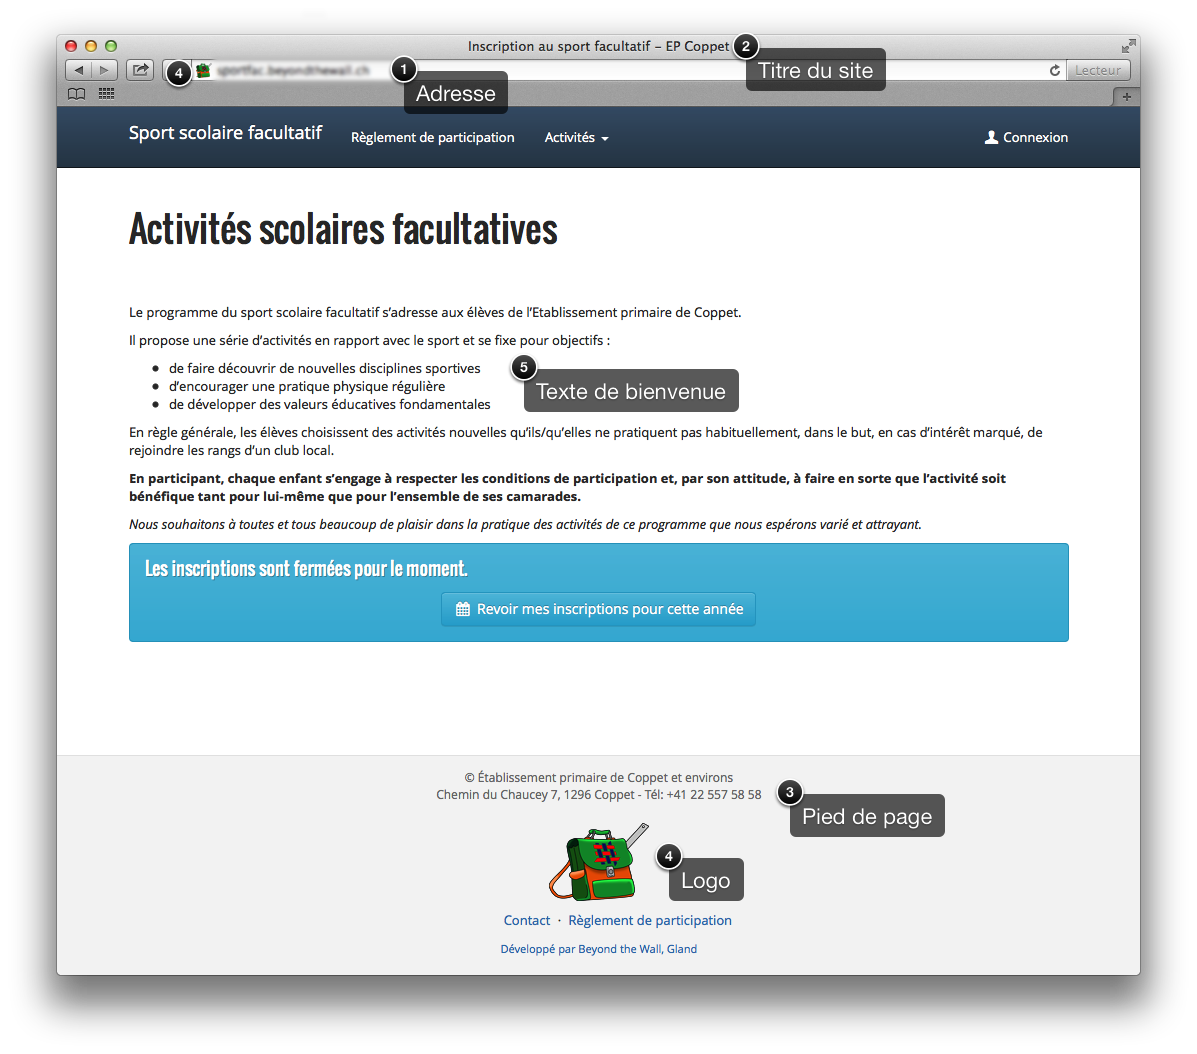
\includegraphics{configure.png}


\section{{[}1{]} Adresse}
\label{configurer:adresse}
L'adresse du site est celle qui sera communiquée aux utilisateurs, sous la forme, par exemple, \href{http://nyon.kepchup.ch}{http://nyon.kepchup.ch}.
Les adresses du type votrenom.ch sont à réserver auprès d'un registrar, par exemple \href{http://gandi.net}{Gandi}.

Les adresses du type votrenom.kepchup.ch sont gratuites.
\begin{itemize}
\item {} 
domaine personnel: \_\_\_\_\_\_\_\_\_\_\_\_\_\_\_\_\_\_\_\_\_

\end{itemize}

ou
\begin{itemize}
\item {} 
sous domaine de kepchup: \_\_\_\_\_\_\_\_\_\_\_\_\_\_\_\_\_.kepchup.ch

\end{itemize}


\section{Personnalisation du site}
\label{configurer:personnalisation-du-site}\begin{itemize}
\item {} 
{[}2{]} Titre du site: Il apparait dans la barre de titre du navigateur sur chaque page.

\end{itemize}
\begin{quote}\begin{description}
\item[{Exemple}] \leavevmode
\begin{DUlineblock}{0em}
\item[] Inscription au sport facultatif - EP Coppet
\end{DUlineblock}

\end{description}\end{quote}
\begin{itemize}
\item {} 
{[}3{]} Pied de page: il est identique sur toutes les pages. On y place généralement le nom et l'adresse de contact, ainsi qu'un logo.

\end{itemize}
\begin{quote}\begin{description}
\item[{Exemple}] \leavevmode
\begin{DUlineblock}{0em}
\item[] © Établissement primaire de Coppet et environs
\item[] Chemin du Chaucey 7, 1296 Coppet - Tél: +41 22 557 58 58
\item[] 
\item[] {[}logo{]}
\end{DUlineblock}

\end{description}\end{quote}
\begin{itemize}
\item {} 
{[}4{]} Logo: utilisé dans le pied de page, en petit dans la barre d'adresse.

\end{itemize}


\subsection{Page d'accueil}
\label{configurer:page-d-accueil}
{[}5{]} Texte de bienvenue, visible sur la page d'accueil.
\begin{quote}\begin{description}
\item[{Exemple}] \leavevmode
\begin{DUlineblock}{0em}
\item[] Le programme du sport scolaire facultatif s’adresse aux élèves de l’Etablissement primaire de Coppet.
\item[] 
\item[] Il propose une série d’activités en rapport avec le sport et se fixe pour objectifs :
\item[]
\begin{DUlineblock}{\DUlineblockindent}
\item[] * de faire découvrir de nouvelles disciplines sportives
\item[] * d’encourager une pratique physique régulière
\item[] * de développer des valeurs éducatives fondamentales
\end{DUlineblock}
\item[] En règle générale, les élèves choisissent des activités nouvelles qu’ils/qu’elles ne pratiquent pas habituellement, dans le but, en cas d’intérêt marqué, de rejoindre les rangs d’un club local.
\item[] 
\item[] \textbf{En participant, chaque enfant s’engage à respecter les conditions de participation et, par son attitude, à faire en sorte que l’activité soit bénéfique tant pour lui-même que pour l’ensemble de ses camarades.}
\item[] 
\item[] \emph{Nous souhaitons à toutes et tous beaucoup de plaisir dans la pratique des activités de ce programme que nous espérons varié et attrayant.}
\end{DUlineblock}

\end{description}\end{quote}


\subsection{Page de contact}
\label{configurer:page-de-contact}
À droite du formulaire de contact se trouvent les coordonnées complètes. \href{http://kepchup.ch/contact/}{http://kepchup.ch/contact/}
\begin{quote}\begin{description}
\item[{Exemple}] \leavevmode
\begin{DUlineblock}{0em}
\item[] \textbf{Établissement Primaire de Coppet et Environs}
\item[] 
\item[] Chemin du Chaucey 7
\item[] CH-1296 Coppet
\item[] \textbf{Téléphone}  +41 22 557 58 58
\item[] \textbf{Fax} +41 22 557 58 59
\item[] \textbf{Email} \href{mailto:ep.coppet@vd.ch}{ep.coppet@vd.ch}
\item[] 
\item[] 
\item[] \textbf{Responsable Sport Scolaire Facultatif}
\item[] 
\item[] Remo Aeschbach
\item[] Chemin du Chaucey 7
\item[] CH-1296 Coppet
\item[] \textbf{Téléphone} +41 22 557 58 58
\item[] \textbf{Portable} +41 79 417 69 93
\item[] \textbf{Email} \href{mailto:remo.aeschbach@vd.educanet2.ch}{remo.aeschbach@vd.educanet2.ch}
\end{DUlineblock}

\end{description}\end{quote}


\subsection{Page du règlement de participation}
\label{configurer:page-du-reglement-de-participation}
Un règlement de participation est à prévoir. À titre d'exemple, celui de Coppet: \href{http://kepchup.ch/reglement/}{http://kepchup.ch/reglement/}


\subsection{Page des paiements}
\label{configurer:page-des-paiements}
Les utilisateurs paient par virement bancaire, ou en apportant l'argent directement. Il n'y a pas de système de paiement en ligne pour le moment.
\begin{itemize}
\item {} 
Texte d'explication.

\end{itemize}
\begin{quote}\begin{description}
\item[{Exemple}] \leavevmode
\begin{DUlineblock}{0em}
\item[] Nous vous remercions de verser cette somme d’ici au  \{\{ registration\_end\textbar{}date:''j F Y'' \}\} en privilégiant le virement bancaire sur le compte :
\item[] IBAN: CH77 0076 7000 C507 0682 4
\item[] Adresse: AIC, 1201 Genève
\end{DUlineblock}

\end{description}\end{quote}


\section{Emails}
\label{configurer:emails}
Beaucoup d'emails peuvent être envoyés par le système: rappel d'inscription, de paiement, liste des participants d'un cours, etc.
\begin{itemize}
\item {} 
Adresse utilisée pour l'envoi des emails automatiques

\item {} 
Signature au bas de chaque email automatique, par exemple:

\end{itemize}
\begin{quote}\begin{description}
\item[{Exemple}] \leavevmode
\begin{DUlineblock}{0em}
\item[] Remo Aeschbach
\item[] Doyen - responsable du sport scolaire facultatif
\item[] EPCoppet
\item[] Chemin du Chaucey 7
\item[] 1296 Coppet
\item[] \href{mailto:remo.aeschbach@vd.educanet2.ch}{remo.aeschbach@vd.educanet2.ch}
\item[] +4122 \textbar{} 557 58 58
\item[] +4179 \textbar{} 417 69 93
\end{DUlineblock}

\end{description}\end{quote}


\subsection{Fin des inscriptions}
\label{configurer:fin-des-inscriptions}
Email envoyé aux utilisateurs qui ont commencé leur inscription, mais ne l'ont pas terminée.
\begin{quote}\begin{description}
\item[{Sujet}] \leavevmode
Votre inscription au sport scolaire facultatif​​​​

\item[{Message}] \leavevmode
\begin{DUlineblock}{0em}
\item[] Madame, Monsieur,
\item[] 
\item[] En passant en revue les inscriptions aux sports scolaires facultatifs, nous constatons que les inscriptions pour votre/vos enfant/s ne sont à ce jour pas encore confirmées (passage à l'étape du paiement).
\item[] 
\item[] Nous vous serions reconnaissants de bien vouloir contrôler les inscriptions que vous avez saisies, de les modifier si nécessaire et de confirmer d'ici à demain soir afin que nous puissions terminer le processus d'inscription.
\item[] 
\item[] Le site des inscriptions: \href{http://votrenom.com}{http://votrenom.com}
\item[] 
\item[] Enfin, nous vous saurions gré de verser le montant relatif à ces inscriptions sur le compte indiqué.
\item[] En vous remerciant de votre collaboration, nous vous adressons nos cordiaux messages.
\end{DUlineblock}

\end{description}\end{quote}


\subsection{​Rappel de paiement}
\label{configurer:rappel-de-paiement}
Envoyé aux utilisateurs qui n'ont pas encore payé. Le montant dû est calculé en fonction de l'utilisateur.
\begin{quote}\begin{description}
\item[{Sujet}] \leavevmode
Votre inscription au sport scolaire facultatif​​​​ - Rappel

\item[{Message}] \leavevmode
\begin{DUlineblock}{0em}
\item[] Madame, Monsieur,
\item[] 
\item[] À ce jour jour et sauf erreur de notre part, nous n’avons pas reçu votre paiement pour les activités de sport scolaire facultatif de votre enfant.
\item[] Nous vous saurions gré d’effectuer votre versement:
\item[] 
\item[] total dû: CHF xxx.-
\item[] 
\item[] sur le compte :
\item[] IBAN: CH77 0076 7000 C507 0682 4
\item[] Adresse: AIIP, 1201 Genève
\item[] 
\item[] en précisant votre identifiant dans les communications: xxx
\item[] 
\item[] Vous pouvez également passer à notre secrétariat (avec une copie imprimée du présent mail) qui pourra encaisser directement votre finance d’inscription.
\item[] En vous remerciant d’ores et déjà de votre prompte réaction, nous vous adressons nos cordiaux messages.
\end{DUlineblock}

\end{description}\end{quote}


\subsection{Infos pour le moniteur}
\label{configurer:infos-pour-le-moniteur}
Les moniteurs des cours reçoivent avant le début de leur cours un email personnalisé contenant divers formulaires (déclaration d'heures pour le canton, liste des participants, feuilles de présence).
\begin{quote}\begin{description}
\item[{Sujet}] \leavevmode
Sport scolaire facultatif - documents monitrice/moniteur cours: {[}N° cours{]} - {[}nom du cours​{]}

\item[{Message}] \leavevmode
\begin{DUlineblock}{0em}
\item[] Chère monitrice, cher moniteur,
\item[] 
\item[] Nous te remercions de t'engager dans l'animation d'une activité du sport scolaire facultatif primaire au sein de notre région et ainsi contribuer à promouvoir la pratique sportive auprès de nos élèves.
\item[] Tu trouveras en pièce jointe tous les documents relatifs au cours dont tu as la charge et qui débute prochainement :
\item[] 
\item[] • liste de tous les cours organisés, avec les informations détaillées de lieux, dates et heures
\item[] • liste des participants avec les n° en cas d'urgence
\item[] • liste de présence à retourner dès la fin du cours
\item[] • feuille de décompte monitrice/moniteur, à retourner dès la fin du cours également
\item[] 
\item[] Tu as la responsabilité de prendre toutes les mesures nécessaires lors d'une absence éventuelle à l'une ou l'autre de tes leçons, soit :
\item[] 
\item[] • dans toute la mesure du possible, te faire remplacer par une personne compétente
\item[] • dans l'impossibilité de te faire remplacer, prévenir tous les participants afin d'éviter le déplacement inutile de ces derniers sur le lieu du cours
\item[] • communiquer ton absence au secrétariat primaire (022-557.58.58)
\item[] 
\item[] Afin que nous puissions te régler dans les meilleurs délais, nous te prions de nous retourner, dès la fin d'un cours, mais au plus tard à la fin de l'année scolaire, les documents suivants, dûment complétés :
\item[] 
\item[] • feuille de décompte, à compléter à l'écran, imprimer et signer - 1 feuille par cours et par monitrice/moniteur
\item[] • liste de présence
\item[] 
\item[] Nous restons à ta disposition pour tout complément d'information, te souhaitons bonne réception de ce courriel et plein succès dans ces activités.
\item[] 
\item[] Meilleurs messages,
\end{DUlineblock}

\end{description}\end{quote}


\subsection{Début d'un cours}
\label{configurer:debut-d-un-cours}
Les parents sont informés par un mail personnalisé pour chacune de leur inscriptions.
\begin{quote}\begin{description}
\item[{Sujet}] \leavevmode
Sport scolaire facultatif - documents monitrice/moniteur cours: {[}N° cours{]} - {[}nom du cours​{]}

\item[{Message}] \leavevmode
\begin{DUlineblock}{0em}
\item[] Madame, Monsieur,
\item[] 
\item[] Nous avons le plaisir d'inviter votre enfant {[}Prénom et nom de l'enfant{]} à la première séance du cours suivant :
\item[] 
\item[] {[}nom du cours{]}
\item[] Responsable : {[}nom du moniteur{]}
\item[] Jour : {[}jour de la semaine{]} de {[}heure de début{]} à {[}heure de fin{]}
\item[] Date 1ère séance : {[}date{]}
\item[] Nombre de séances : {[}nombre{]}
\item[] Rendez-vous/lieu du cours : {[}lieu{]}
\item[] 
\item[] L'animatrice/l'animateur vous donnera toutes les informations en lien avec son cours lors de la 1ère séance.
\item[] 
\item[] En restant à votre disposition pour tout complément d'information, nous vous adressons, Madame, Monsieur, nos cordiaux messages.
\end{DUlineblock}

\end{description}\end{quote}


\section{Admininistrateur}
\label{configurer:admininistrateur}
Une personne au moins devra être administrateur du site.
\begin{itemize}
\item {} 
Prénom

\item {} 
Nom

\item {} 
email

\end{itemize}


\chapter{Indices and tables}
\label{index:indices-and-tables}\begin{itemize}
\item {} 
\DUspan{xref,std,std-ref}{genindex}

\item {} 
\DUspan{xref,std,std-ref}{modindex}

\item {} 
\DUspan{xref,std,std-ref}{search}

\end{itemize}



\renewcommand{\indexname}{Index}
\printindex
\end{document}
